% !TeX program = xelatex
% !TeX options = -shell-escape
% !TEX encoding = UTF-8

% --------------------------------------------------------------
% This is all preamble stuff that you don't have to worry about.
% Head down to where it says "Start here"
% --------------------------------------------------------------

\documentclass[12pt]{article}
\usepackage[margin=2cm]{geometry} % 頁面邊距設置
\usepackage{amsmath,amssymb,amsthm} % 數學相關套件
\usepackage{graphicx} % 圖形插入
\usepackage{booktabs} % 表格線條
\usepackage[AutoFakeBold,AutoFakeSlant]{xeCJK} % 中文支援
\usepackage{fancyhdr} % 頁首頁尾設置
\usepackage{xcolor,changepage,mdframed} % 顏色與框線相關
\usepackage{titlesec} % 標題格式
\usepackage{setspace} % 行距
\usepackage{minted} % 程式碼高亮（需安裝 Python 套件 pygments）
\usepackage[shortlabels]{enumitem} % 列表格式
\usepackage[colorlinks=true,linkcolor=black,urlcolor=blue,citecolor=blue]{hyperref} % 超連結
\graphicspath{{images}}

% 字體設定 (xeCJK)
\setCJKmainfont{黑體-繁}
\setCJKmonofont{Noto Sans CJK TC}

% 頁首/頁尾設定 (fancyhdr)
\pagestyle{fancy}
\fancyhead[L]{NASA Homework 2} % 可以用 \leftmark 取代
\fancyhead[R]{B13901011 吳亞倫}
\fancyfoot[C]{\thepage}
\renewcommand{\headrulewidth}{0.4pt}
\renewcommand{\footrulewidth}{0pt}
\setlength{\headheight}{15pt}

% tex-fmt: off
\newtheorem*{theorem}{Theorem}
\newenvironment{lemma}[2][Lemma]{\begin{trivlist}
\item[\hskip \labelsep {\bfseries #1}\hskip \labelsep {\bfseries #2.}]}{\end{trivlist}}
\newenvironment{exercise}[2][Exercise]{\begin{trivlist}
\item[\hskip \labelsep {\bfseries #1}\hskip \labelsep {\bfseries #2.}]}{\end{trivlist}}
\newenvironment{problem}[2][Problem]{\begin{trivlist}
\item[\hskip \labelsep {\bfseries #1}\hskip \labelsep {\bfseries #2}]}{\end{trivlist}}
\newenvironment{question}[2][Question]{\begin{trivlist}
\item[\hskip \labelsep {\bfseries #1}\hskip \labelsep {\bfseries #2.}]}{\end{trivlist}}
\newenvironment{corollary}[2][Corollary]{\begin{trivlist}
\item[\hskip \labelsep {\bfseries #1}\hskip \labelsep {\bfseries #2.}]}{\end{trivlist}}
\newenvironment{solution}{\begin{proof}[Solution]}{\end{proof}}
\newenvironment{answer}{\begin{proof}[Ans]}{\end{proof}}

% 樣式設定
\renewcommand\thesubsection{\arabic{subsection}}
\titleformat{\subsection}{\normalfont\large\bfseries}{\thesubsection.}{0.5em}{}
\renewcommand{\thesection}{\arabic{section}.}
\setminted{frame=lines, linenos, framesep=2mm, breaklines=true, breakanywhere=true, autogobble=true}

% 自訂框線環境
\newmdenv[
  linewidth=2pt, linecolor=gray, backgroundcolor=gray!10,
  topline=false, bottomline=false, rightline=false,
  skipabove=10pt, skipbelow=10pt, innerleftmargin=10pt,
  innerrightmargin=0pt, innertopmargin=5pt, innerbottommargin=5pt
]{myquote}

\newenvironment{mycolorbox}[1][gray]{
  \renewmdenv[
    linewidth=2pt, linecolor=#1, backgroundcolor=#1!10,
    topline=false, bottomline=false, rightline=false,
    skipabove=10pt, skipbelow=10pt, innerleftmargin=10pt,
    innerrightmargin=0pt, innertopmargin=5pt, innerbottommargin=5pt
  ]{myquote}
  \begin{myquote}
}{\end{myquote}}

\linespread{1.1}
% \usemintedstyle{xcode}
\AtBeginEnvironment{minted}{\vspace{-10pt}} % 可根據需求調整間距數值
\setminted{breaklines=true, breakanywhere=true, autogobble=true}

% tex-fmt: on
\begin{document}
\thispagestyle{fancy}

%------------------------------------------------------------
%                         Start here
% -----------------------------------------------------------

\begin{center}
  {\large \bfseries Network Administration / System Administration} \\
  \vspace{1em}
  {\Large \bfseries Homework 2} \\
\end{center}

\vspace{2em}

\begin{tabular}{@{}l l}
  \textbf{Student:} & 吳亞倫 \\
  \textbf{ID:} & B13901011  \\
  \textbf{Department:} & 電機工程學系
\end{tabular}
\bigskip

\begin{mycolorbox}[cyan]
  \textbf{Discussion Partners:}
  \begin{itemize}
    \item Classmates：賴泓安、鄭竣陽、陳澔樂、喻慈恩
      \vspace{0.5em}
  \end{itemize}
\end{mycolorbox}

\setcounter{section}{-1}

% -----------------------------------------------------------
% Problem 0
\section{VM Setup}
\begin{mycolorbox}[teal]
  \textbf{Reference:}
  \footnotesize
  \begin{itemize}
    \item \href{https://bbs.archlinux.org/viewtopic.php?id=303841}{unable to retrieve community.db: 404 errors (Arch Linux Forums)}
    \item \href{https://unix.stackexchange.com/questions/574493/sudo-pacman-syu-fails-with-error-failed-to-commit-transaction-invalid-or-cor}{sudo pacman -Syu fails with error: failed to commit transaction (Stack Exchange)}
    \item \href{https://wiki.archlinux.org/title/OpenSSH}{OpenSSH (ArchWiki)}
    \item \href{https://medium.com/@pythonaugust/enable-ssh-on-arch-linux-8f1ede0d9c88}{Enable SSH on Arch Linux}
  \end{itemize}
\end{mycolorbox}
\vspace{0.5em}

為了方便連線，我打算在 VM 當中配置 ssh server，使我可以利用 ssh 的方式進入虛擬機。步驟如下：

\begin{enumerate}
  \item 執行 \texttt{run\_vm.sh}，以 vnc 登入 VM 當中的 root 帳號。
  \item 更新 archlinux 失敗，經查閱資料後，發現需要將 \texttt{/etc/pacman.conf} 中的 \texttt{[[community]]} 註解掉。
  \item 更新 archlinux keyring
  \begin{minted}{bash}
    pacman -Sy archlinux-keyring
  \end{minted}
  \item 更新 archlinux 並安裝 openssh：
  \begin{minted}{bash}
  pacman -Syu
  pacman -S openssh
  \end{minted}
  \item 啟動 sshd
  \begin{minted}{bash}
    systemctl enable sshd
    systemctl start sshd
  \end{minted}
  \item 離開 VM，並在 host 端修改 \texttt{run\_vm.sh}，加入最後一行，使 host 端的 4321 port 轉發到 VM 的 22 port。
  \begin{minted}{bash}
    #!/bin/bash

    echo "Starting VM at port $1"
    echo "parameter is $(($1 - 5900))"

    qemu-system-x86_64 -m 2G --enable-kvm \
            -vnc :"$(($1 - 5900))",password=on -monitor stdio \
            -drive file=disk1.qcow2,media=disk,index=0 \
            -drive file=disk2.qcow2,if=virtio,media=disk,index=1 \
            -drive file=disk3.qcow2,if=virtio,media=disk,index=2 \
            -drive file=disk4.qcow2,if=virtio,media=disk,index=3 \
            -drive file=disk5.qcow2,if=virtio,media=disk,index=4 \
            -drive file=disk6.qcow2,if=virtio,media=disk,index=5 \
            -drive file=disk7.qcow2,if=virtio,media=disk,index=6 \
            -drive file=disk8.qcow2,if=virtio,media=disk,index=7 \
            -drive file=disk9.qcow2,if=virtio,media=disk,index=8 \
            -drive file=disk10.qcow2,if=virtio,media=disk,index=9 \
            -net user,hostfwd=tcp::4321-:22 -net nic
  \end{minted}
  \item 成功從工作站當中以 balu 的帳號 ssh 進去 VM。
  \begin{minted}{bash}
    ssh balu@localhost -p 4321
  \end{minted}
\end{enumerate}

% -----------------------------------------------------------
% Problem 1
\section{那傢伙竟然敢無視窗}

\begin{mycolorbox}[teal]
  \textbf{Reference:}
  \footnotesize
  \begin{itemize}
    \item \href{https://docs.kernel.org/filesystems/ntfs3.html}{NTFS3}
    \item \href{https://en.wikipedia.org/wiki/Journaling_file_system}{Journaling file system (Wikipedia)}
    \item \href{https://stackoverflow.com/questions/73065519/how-to-mount-ntfs-in-linux-without-fuseblk}{How to mount NTFS in Linux without fuseblk (Stack Overflow)}
    \item \href{https://www.insidentally.com/articles/000029/}{使用 ntfs3 驱动替换 ntfs-3g 挂载 windows NTFS 分区}
    \item \href{https://blog.csdn.net/weixin_43801670/article/details/125105727}{对NTFS硬盘进行读写操作；开机自动挂载硬盘 (CSDN)}
  \end{itemize}
\end{mycolorbox}

NTFS 檔案系統可以滿足題目所要求，在雙系統中支援原生讀寫，並且在 Windows 11 下支援日誌功能。為了格式化 NTFS 檔案系統，需要先安裝 \texttt{ntfs-3g} 套件。我完成此題的步驟如下：

\begin{enumerate}
  \item 在 VM 當中安裝 \texttt{ntfs-3g} 套件
  \begin{minted}{bash}
    sudo pacman -S ntfs-3g
  \end{minted}
  \item 創立掛載點
  \begin{minted}{bash}
    sudo mkdir /mnt/myusb
  \end{minted}
  \item 格式化硬碟
  \begin{minted}{bash}
    sudo mkfs.ntfs /dev/vdi2
  \end{minted}
  \item 取得 UUID
  \begin{minted}{bash}
    sudo blkid /dev/vdi2
  \end{minted}
    \begin{figure}[H]
      \centering
      
\includegraphics[width=\textwidth]{images/1-1.png}
      \caption{Screenshot of \texttt{sudo blkid /dev/vdi2}}
    \end{figure}

  \item 配置自動掛載硬碟: 修改 /etc/fstab
  \item 重開機，即可看到硬碟已經掛載
\end{enumerate}
\begin{mycolorbox}[green]
  \begin{answer} 　
    \begin{figure}[H]
      
\includegraphics[width=0.98\textwidth]{images/1-3.png}
      \caption{Screenshot of \texttt{cat /etc/fstab}}
    \end{figure}

    \begin{figure}[H]
      
\includegraphics[width=0.98\textwidth]{images/1-2.png}
      \caption{Screenshot of \texttt{lsblk; df -hT}}
    \end{figure}
  \end{answer}
\end{mycolorbox}

\clearpage
% -----------------------------------------------------------
% Problem 2
\section{因為要換到新的 SWAP}

\begin{mycolorbox}[teal]
  \textbf{Reference:}
  \footnotesize
  \begin{itemize}
    \item \href{https://linuxize.com/post/create-a-linux-swap-file/}{Create a Linux Swap File (Linuxize)}
  \end{itemize}
\end{mycolorbox}

新增 SWAP 檔案的步驟如下：
\begin{enumerate}
  \item 建立 /newswap 檔案
  \begin{minted}{bash}
    sudo fallocate -l 4G /newswap
  \end{minted}
  \item 設定檔案權限
  \begin{minted}{bash}
    sudo chmod 600 /newswap
  \end{minted}
  \item 格式化檔案
  \begin{minted}{bash}
    sudo mkswap /newswap
  \end{minted}
  \item 啟用 SWAP 檔案
  \begin{minted}{bash}
    sudo swapon /newswap
  \end{minted}
\end{enumerate}

\begin{mycolorbox}[green]
  \begin{answer} 　
    \begin{figure}[H]
      
\includegraphics[width=0.98\textwidth]{images/2-1.png}
      \caption{Screenshot of \texttt{free -h}}
    \end{figure}
  \end{answer}
\end{mycolorbox}

\clearpage
% -----------------------------------------------------------
% Problem 3
\section{為資料創造新的棲身之處}

\begin{mycolorbox}[teal]
  \textbf{Reference:}
  \footnotesize
  \begin{itemize}
    \item \href{https://www.linuxcool.com/lvextend}{lvextend命令 (LinuxCool)}
  \end{itemize}
\end{mycolorbox}
使用指令如下：
\begin{minted}{bash}
  sudo lvextend -L 1GiB /dev/nasahw2-main/course
\end{minted}
\vspace{-0.1cm}
\begin{mycolorbox}[green]
  \begin{answer} 　
    \begin{figure}[H]
      \centering
      
\includegraphics[width=0.95\textwidth]{images/3-1.png}
      \caption{Screenshot of \texttt{lsblk; df -hT}}
    \end{figure}
  \end{answer}
\end{mycolorbox}

\clearpage
% -----------------------------------------------------------
% Problem 4
\section{我有拜託妳別把我的作業告訴其他人了吧}
\begin{mycolorbox}[teal]
  \textbf{Reference:}
  \footnotesize
  \begin{itemize}
    \item \href{https://medium.com/@allypetitt/how-to-encrypt-a-drive-in-linux-83b3001744f4}{How to Encrypt a Drive in Linux (Medium)}
    \item \href{https://access.redhat.com/solutions/230993}{How to add a passphrase, key, or keyfile to an existing LUKS device (Red Hat)}
    \item \href{https://hkgoldenmra.blogspot.com/2019/12/linux-luks-ext4.html}{Linux 使用 LUKS 加密 Ext4 檔案系統}
  \end{itemize}
\end{mycolorbox}

我做的步驟如下：
\begin{enumerate}
  \item 以 root 進入 VM。
  \item 切出一塊新的 lvm，作為加密區域
  \begin{minted}{bash}
    lvcreate -L 800MiB -n homework nasahw2-main
  \end{minted}
  \item 加密 \texttt{/dev/nasahw2-main/homework}
  \begin{minted}{bash}
    cryptsetup luksFormat /dev/nasahw2-main/homework
  \end{minted}
  \item 開啟加密區域
  \begin{minted}{bash}
    cryptsetup open /dev/nasahw2-main/homework homework
  \end{minted}
  \item 格式化加密區域
  \begin{minted}{bash}
    mkfs.ext4 /dev/mapper/homework
  \end{minted}
  \item 掛載加密區域
  \begin{minted}{bash}
    mount /dev/mapper/homework /home/balu/homework/
  \end{minted}
  \item 設定 keyfile
  \begin{minted}{bash}
    cryptsetup luksAddKey /dev/nasahw2-main/homework /home/balu/lvm_key
  \end{minted}
  \item 設定開機自動解密，在 \texttt{/etc/crypttab} 中加入底下這行：
  \begin{minted}{bash}
    homework /dev/nasahw2-main/homework /home/balu/lvm_key
  \end{minted}
  \item 設定開機自動 mount，在 \texttt{/etc/fstab} 中加入底下這行：
  \begin{minted}{bash}
    /dev/mapper/homework /home/balu/homework ext4 defaults 0 2
  \end{minted}
  \item 重開機，確認加密區域已經掛載
\end{enumerate}

\begin{mycolorbox}[green]
  \begin{answer} 　
    \begin{figure}[H]
      \centering
      
\includegraphics[width=0.99\textwidth]{images/4-1.png}
      \caption{Screenshot of \texttt{lsblk; df -hT}}
    \end{figure}
  \end{answer}
\end{mycolorbox}
\clearpage
% -----------------------------------------------------------
% Problem 5
\section{快照真的好難喔}
\begin{mycolorbox}[teal]
  \textbf{Reference:}
  \footnotesize
  \begin{itemize}
    \item \href{https://ithelp.ithome.com.tw/m/articles/10081811}{LVM系統快照設定教學 (iThome)}
    \item \href{https://blog.csdn.net/qq_36393978/article/details/118221951}{Linux解压缩tar.zst类型文件 (CSDN)}
    \item \href{https://serverfault.com/questions/184983/how-to-keep-or-drop-lvm-snapshot}{How to keep or drop LVM snapshot (Server Fault)}
  \end{itemize}
\end{mycolorbox}

我以 root 進入 VM，並進行以下操作：
\begin{enumerate}
  \item 將 \texttt{/dev/vdc1} 設為 pv，並且加到 \texttt{nasahw2-main} vg 中
  \begin{minted}{bash}
    pvcreate /dev/vdc1
    vgextend nasahw2-main /dev/vdc1
  \end{minted}
  \item 建立 snapshot 的 lv
  \begin{minted}{bash}
    lvcreate -L 1GiB -s -n backup /dev/nasahw2-main/course
  \end{minted}
  \item 掛載 \texttt{/dev/nasahw2-main/backup} 到 \texttt{/mnt/backup}
  \begin{minted}{bash}
    mkdir -p /mnt/backup
    mount /dev/nasahw2-main/backup /mnt/backup
  \end{minted}
  \item \texttt{lsblk} 結果如 \autoref{fig:5-1} 所示。
  \item 進行備份到 tar:
  \begin{minted}{bash}
    tar -I zstd -cvf /home/balu/backup.tar.zst /mnt/backup
  \end{minted}
  \item 卸載 /mnt/backup，並刪除 snapshot。
  \begin{minted}{bash}
    umount /mnt/backup
    lvremove /dev/nasahw2-main/backup
  \end{minted}
  \item 執行 \texttt{lsblk; df -hT}，結果如 \autoref{fig:5-2} 所示。

    \begin{figure}
      \centering
      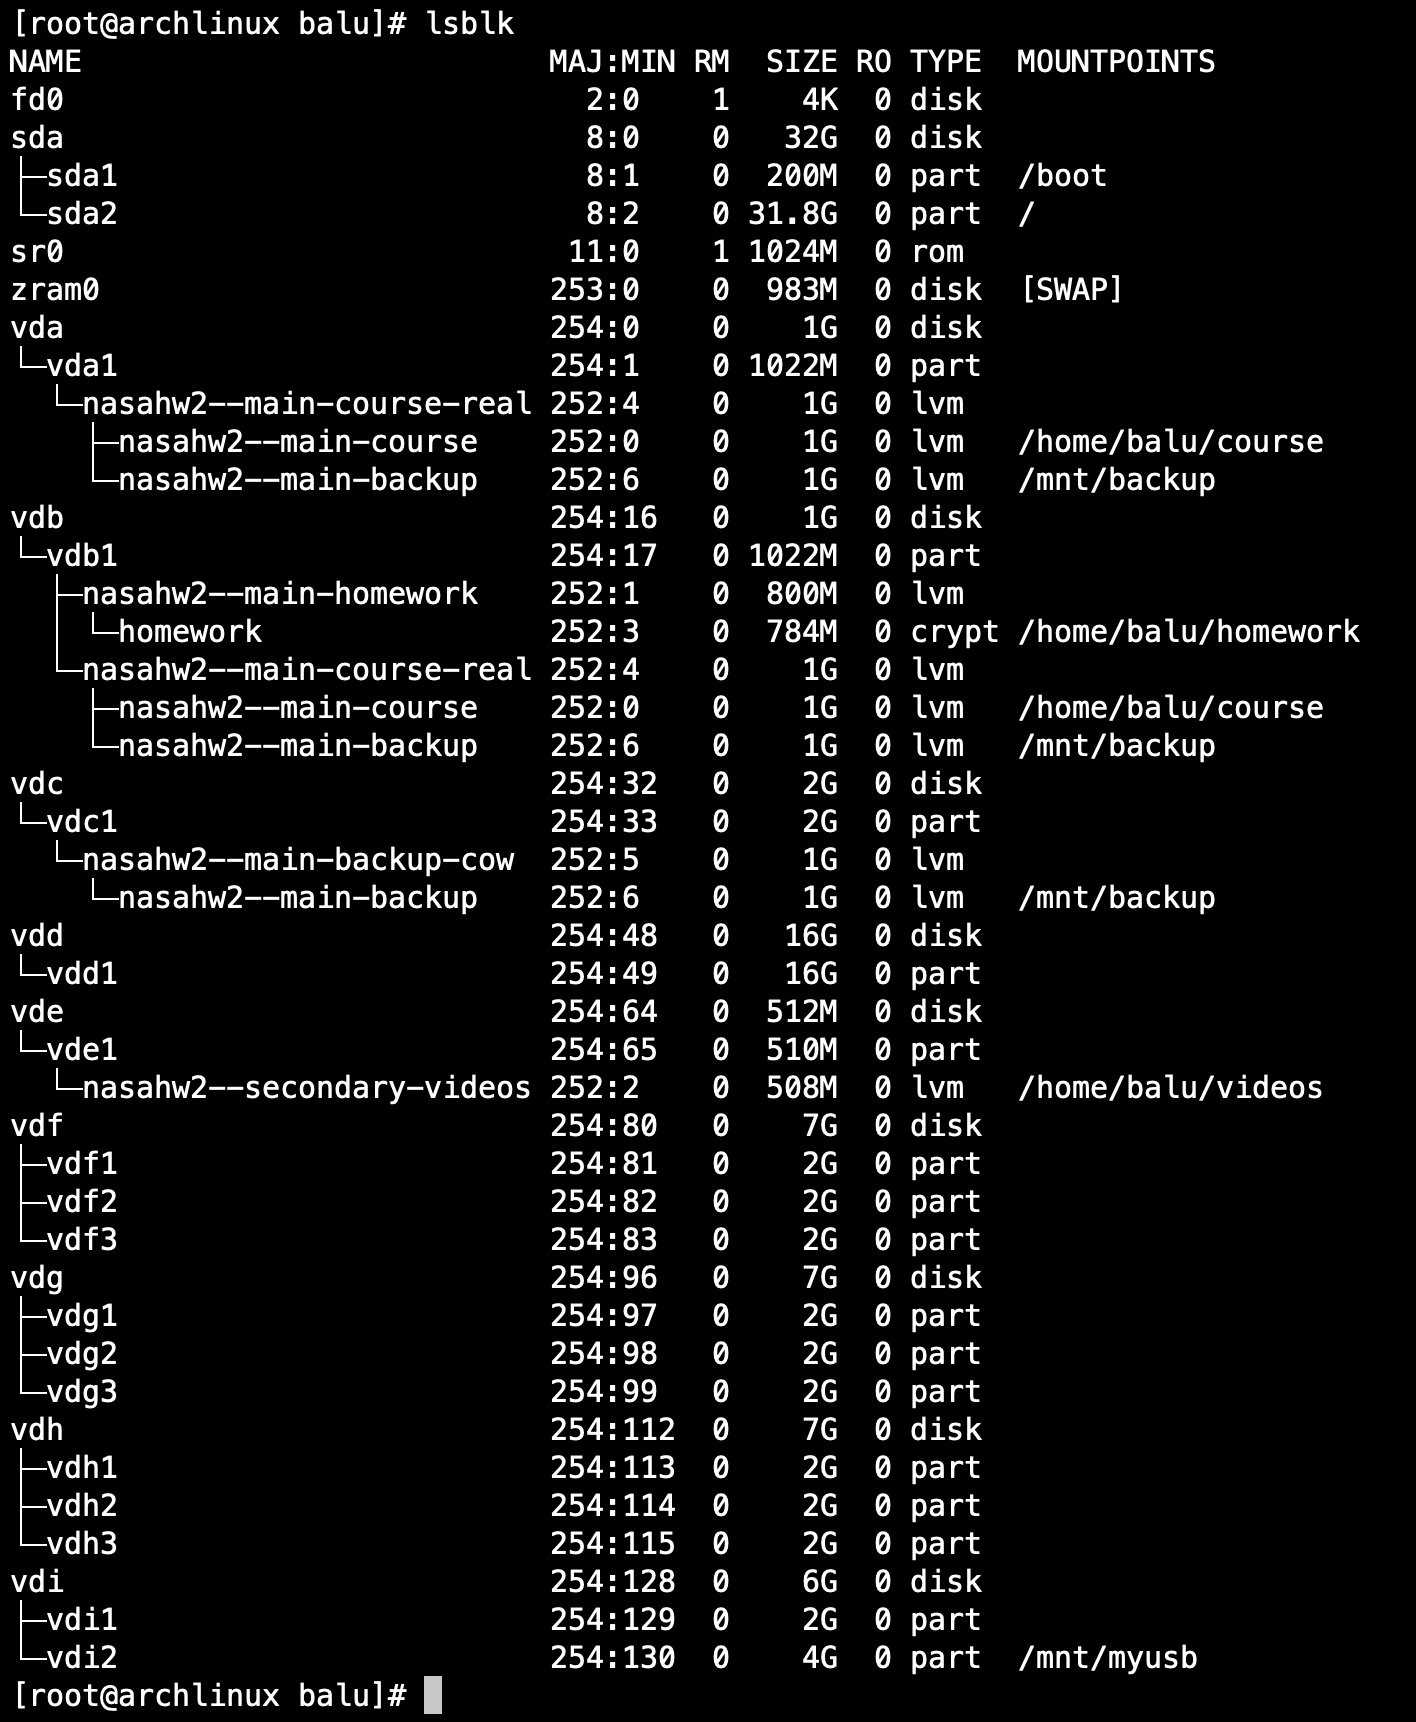
\includegraphics[width=0.95\textwidth]{images/5-1.png}
      \caption{Screenshot of \texttt{lsblk} after creating snapshot}
      \label{fig:5-1}
    \end{figure}

    \begin{figure}
      \centering
      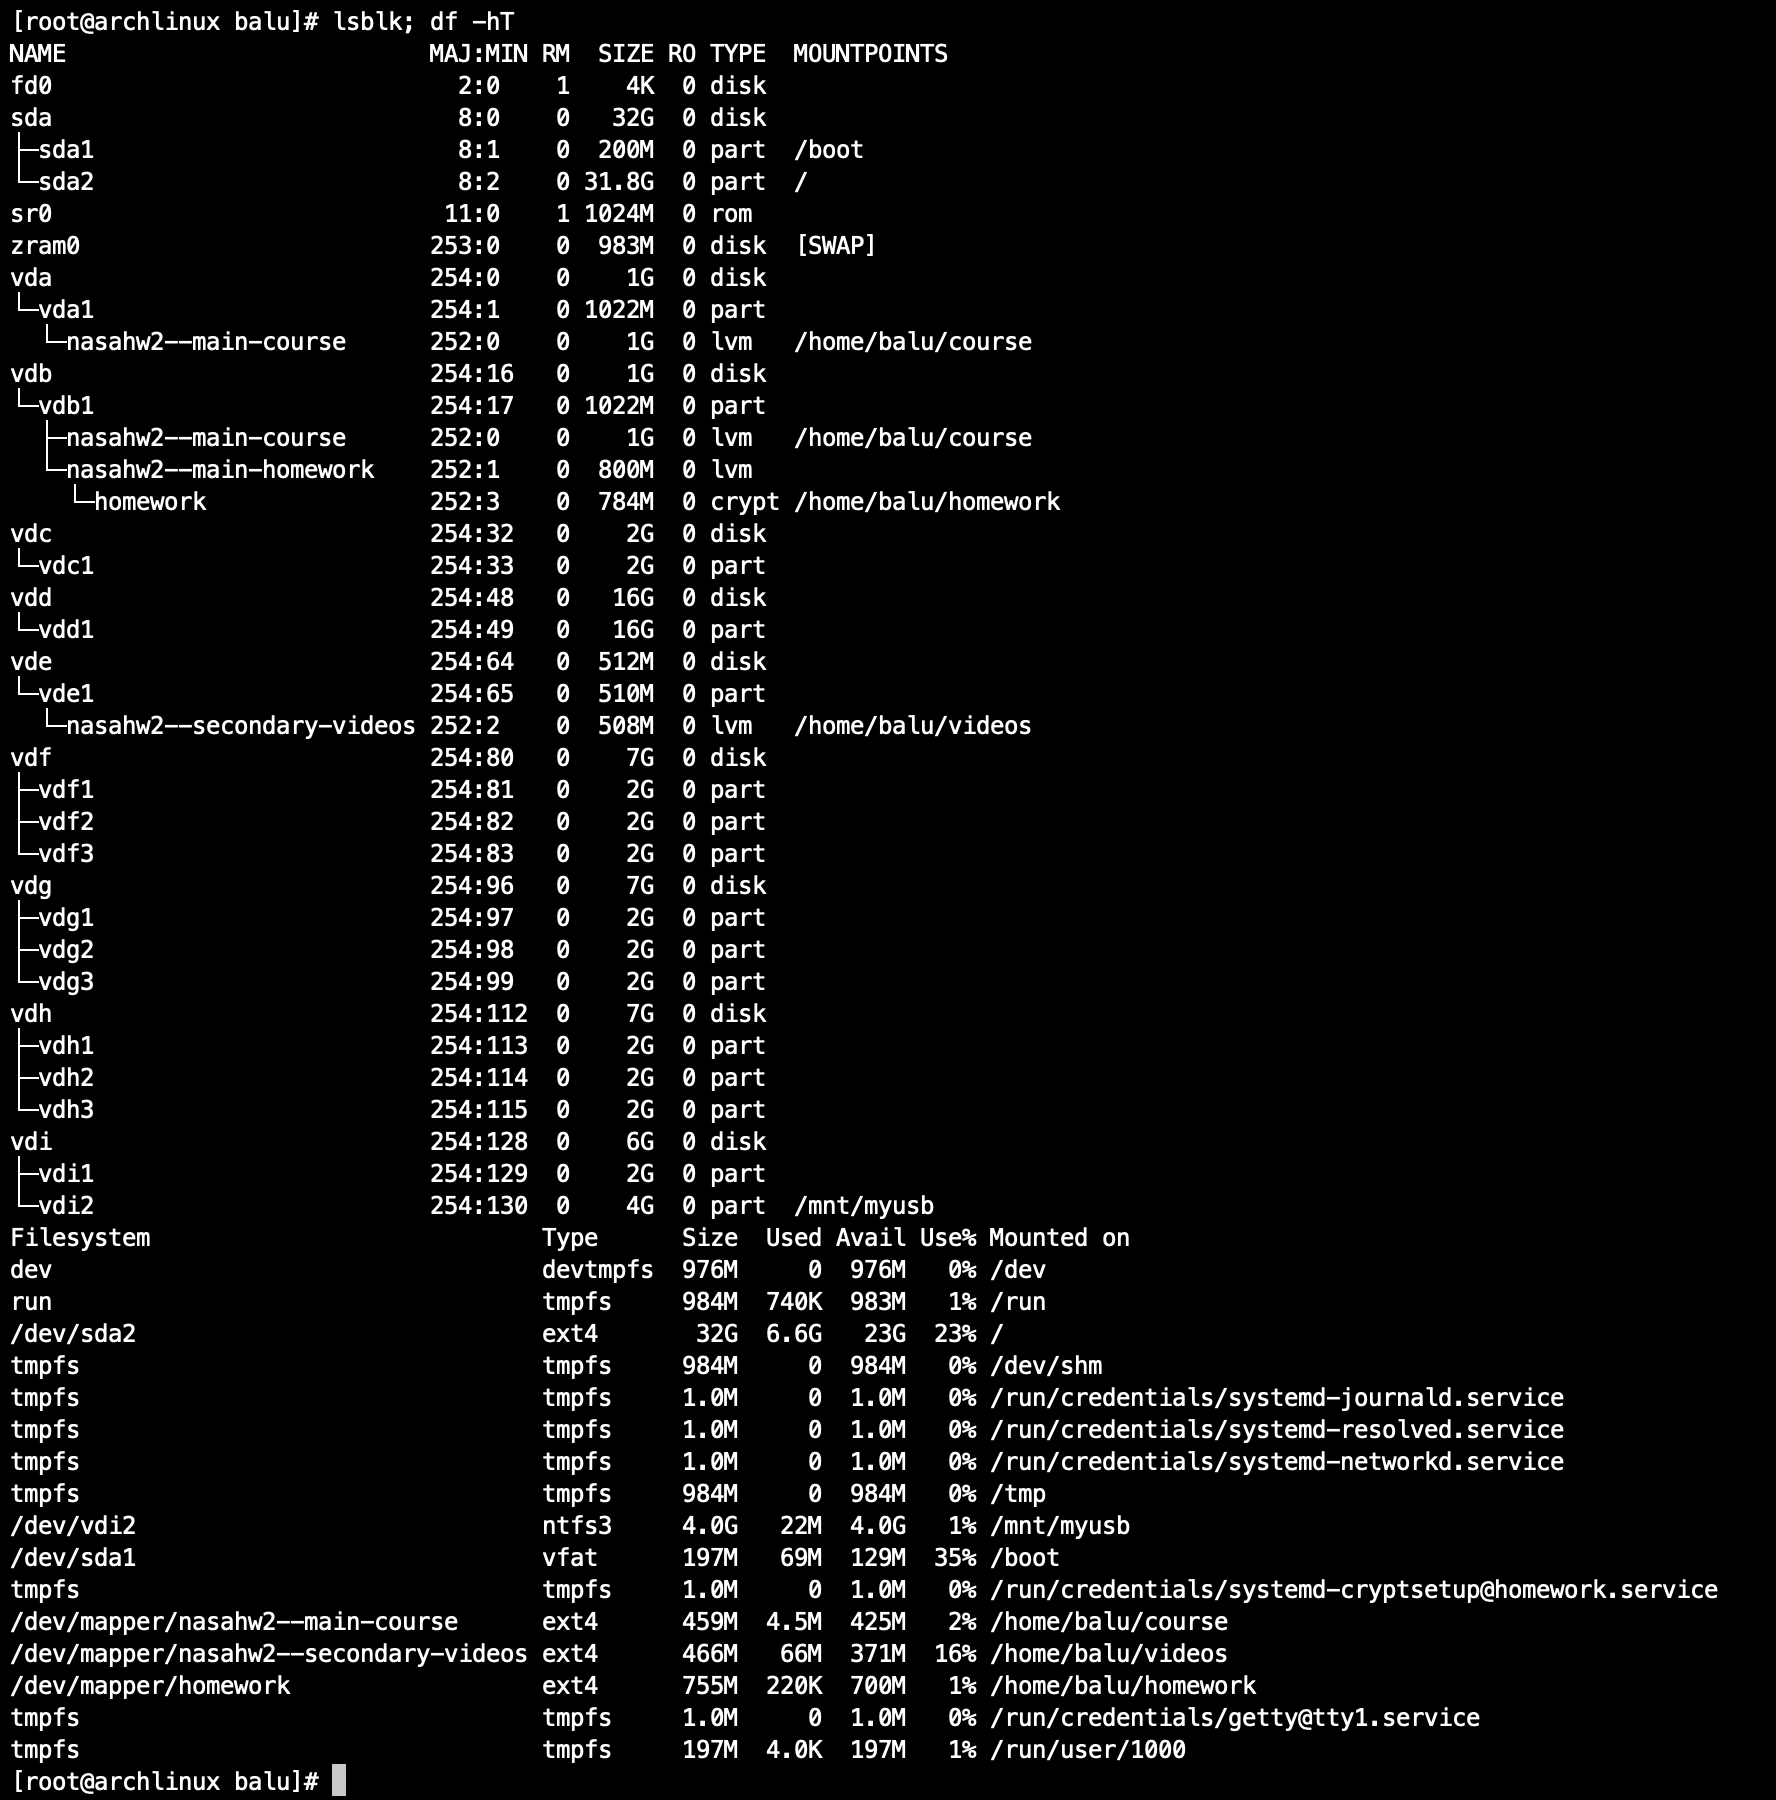
\includegraphics[width=0.95\textwidth]{images/5-2.png}
      \caption{Screenshot of \texttt{lsblk; df -hT} after removing snapshot}
      \label{fig:5-2}
    \end{figure}
\end{enumerate}

\clearpage
% -----------------------------------------------------------
% Problem 6
\section{好老舊喔}

\begin{mycolorbox}[teal]
  \textbf{Reference:}
  \footnotesize
  \begin{itemize}
    \item \href{https://docs.redhat.com/en/documentation/red_hat_enterprise_linux/6/html/logical_volume_manager_administration/vg_remove_pv#VG_remove_PV}{Removing Physical Volumes from a Volume Group (Red Hat)}
    \item \href{https://www.linuxcool.com/pvmove}{pvmove命令 (LinuxCool)}
    \item \href{https://unix.stackexchange.com/questions/679362/remove-a-pv-from-lvm}{Remove a PV from LVM (Stack Exchange)}
  \end{itemize}
\end{mycolorbox}

我以 root 進入 VM，並進行以下操作：
\begin{enumerate}
  \item 將 \texttt{/dev/vdd1} 設為 pv，並且加到 \texttt{nasahw2-secondary} vg 中
  \begin{minted}{bash}
    pvcreate /dev/vdd1
    vgextend nasahw2-secondary /dev/vdd1
  \end{minted}
  \item 搬移 pv \texttt{/dev/vde1} 中的內容到 \texttt{/dev/vdd1}
  \begin{minted}{bash}
    pvmove /dev/vde1 /dev/vdd1
  \end{minted}
  \item 將 \texttt{/dev/vde1} 從 \texttt{nasahw2-secondary} vg 中移除，並且刪除 pv
  \begin{minted}{bash}
    vgreduce nasahw2-secondary /dev/vde1
    pvremove /dev/vde1
  \end{minted}
\end{enumerate}

\begin{mycolorbox}[green]
  \begin{answer} 　
    \begin{figure}[H]
      \centering
      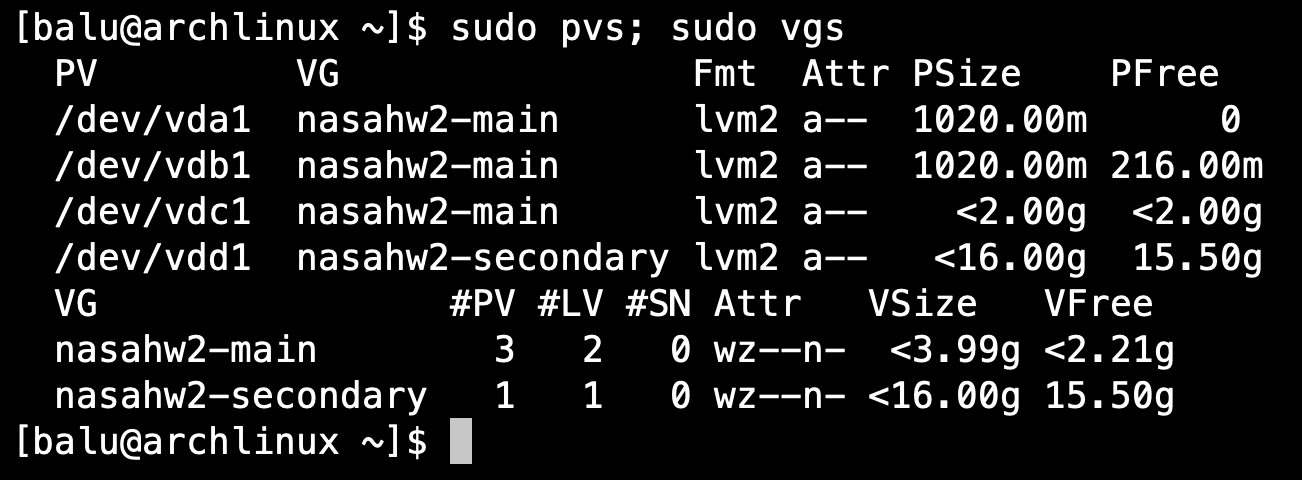
\includegraphics[width=0.95\textwidth]{images/6-1.png}
      \caption{Screenshot of \texttt{sudo pvs; sudo vgs}}
    \end{figure}
  \end{answer}
\end{mycolorbox}

\clearpage
% -----------------------------------------------------------
% Problem 7
\section{我看還是再來合一次吧}

\begin{mycolorbox}[teal]
  \textbf{Reference:}
  \footnotesize
  \begin{itemize}
    \item \href{https://unix.stackexchange.com/questions/190709/merge-2-lvms-both-have-data-and-on-same-volume-group-without-data-loss}{Merge 2 LVs both have data and on same volume group without data loss (Stack Exchange)}
    \item \href{https://docs.redhat.com/zh-cn/documentation/red_hat_enterprise_linux/9/html/configuring_and_managing_logical_volumes/combining-lvm-volume-groups_managing-lvm-volume-groups}{合并 LVM 卷组 (Red Hat)}
  \end{itemize}
\end{mycolorbox}

我以 root 進入 VM，並進行以下操作：
\begin{enumerate}
  \item 將 \texttt{nasahw2-secondary} 的所有磁區都 unmount，並且 deactivate 該 vg。
  \begin{minted}{bash}
    umount /dev/nasahw2-secondary/*
    vgchange -a n nasahw2-secondary
  \end{minted}
  \item 透過 vgmerge -t 測試合併 \texttt{nasahw2-secondary} 到 \texttt{nasahw2-main} 是否會有異常。確認完成後，執行 vgmerge。
  \begin{minted}{bash}
    vgmerge -t nasahw2-main nasahw2-secondary
    vgmerge nasahw2-main nasahw2-secondary
  \end{minted}
  \item 修改開機自動啟動，將 \texttt{/ect/fstab} 當中的 \texttt{nasahw2-secondary} 改為 \texttt{nasahw2-main}
  \item 重開機，確認合併成功
\end{enumerate}

\begin{mycolorbox}[green]
  \begin{answer} 　
    \begin{figure}[H]
      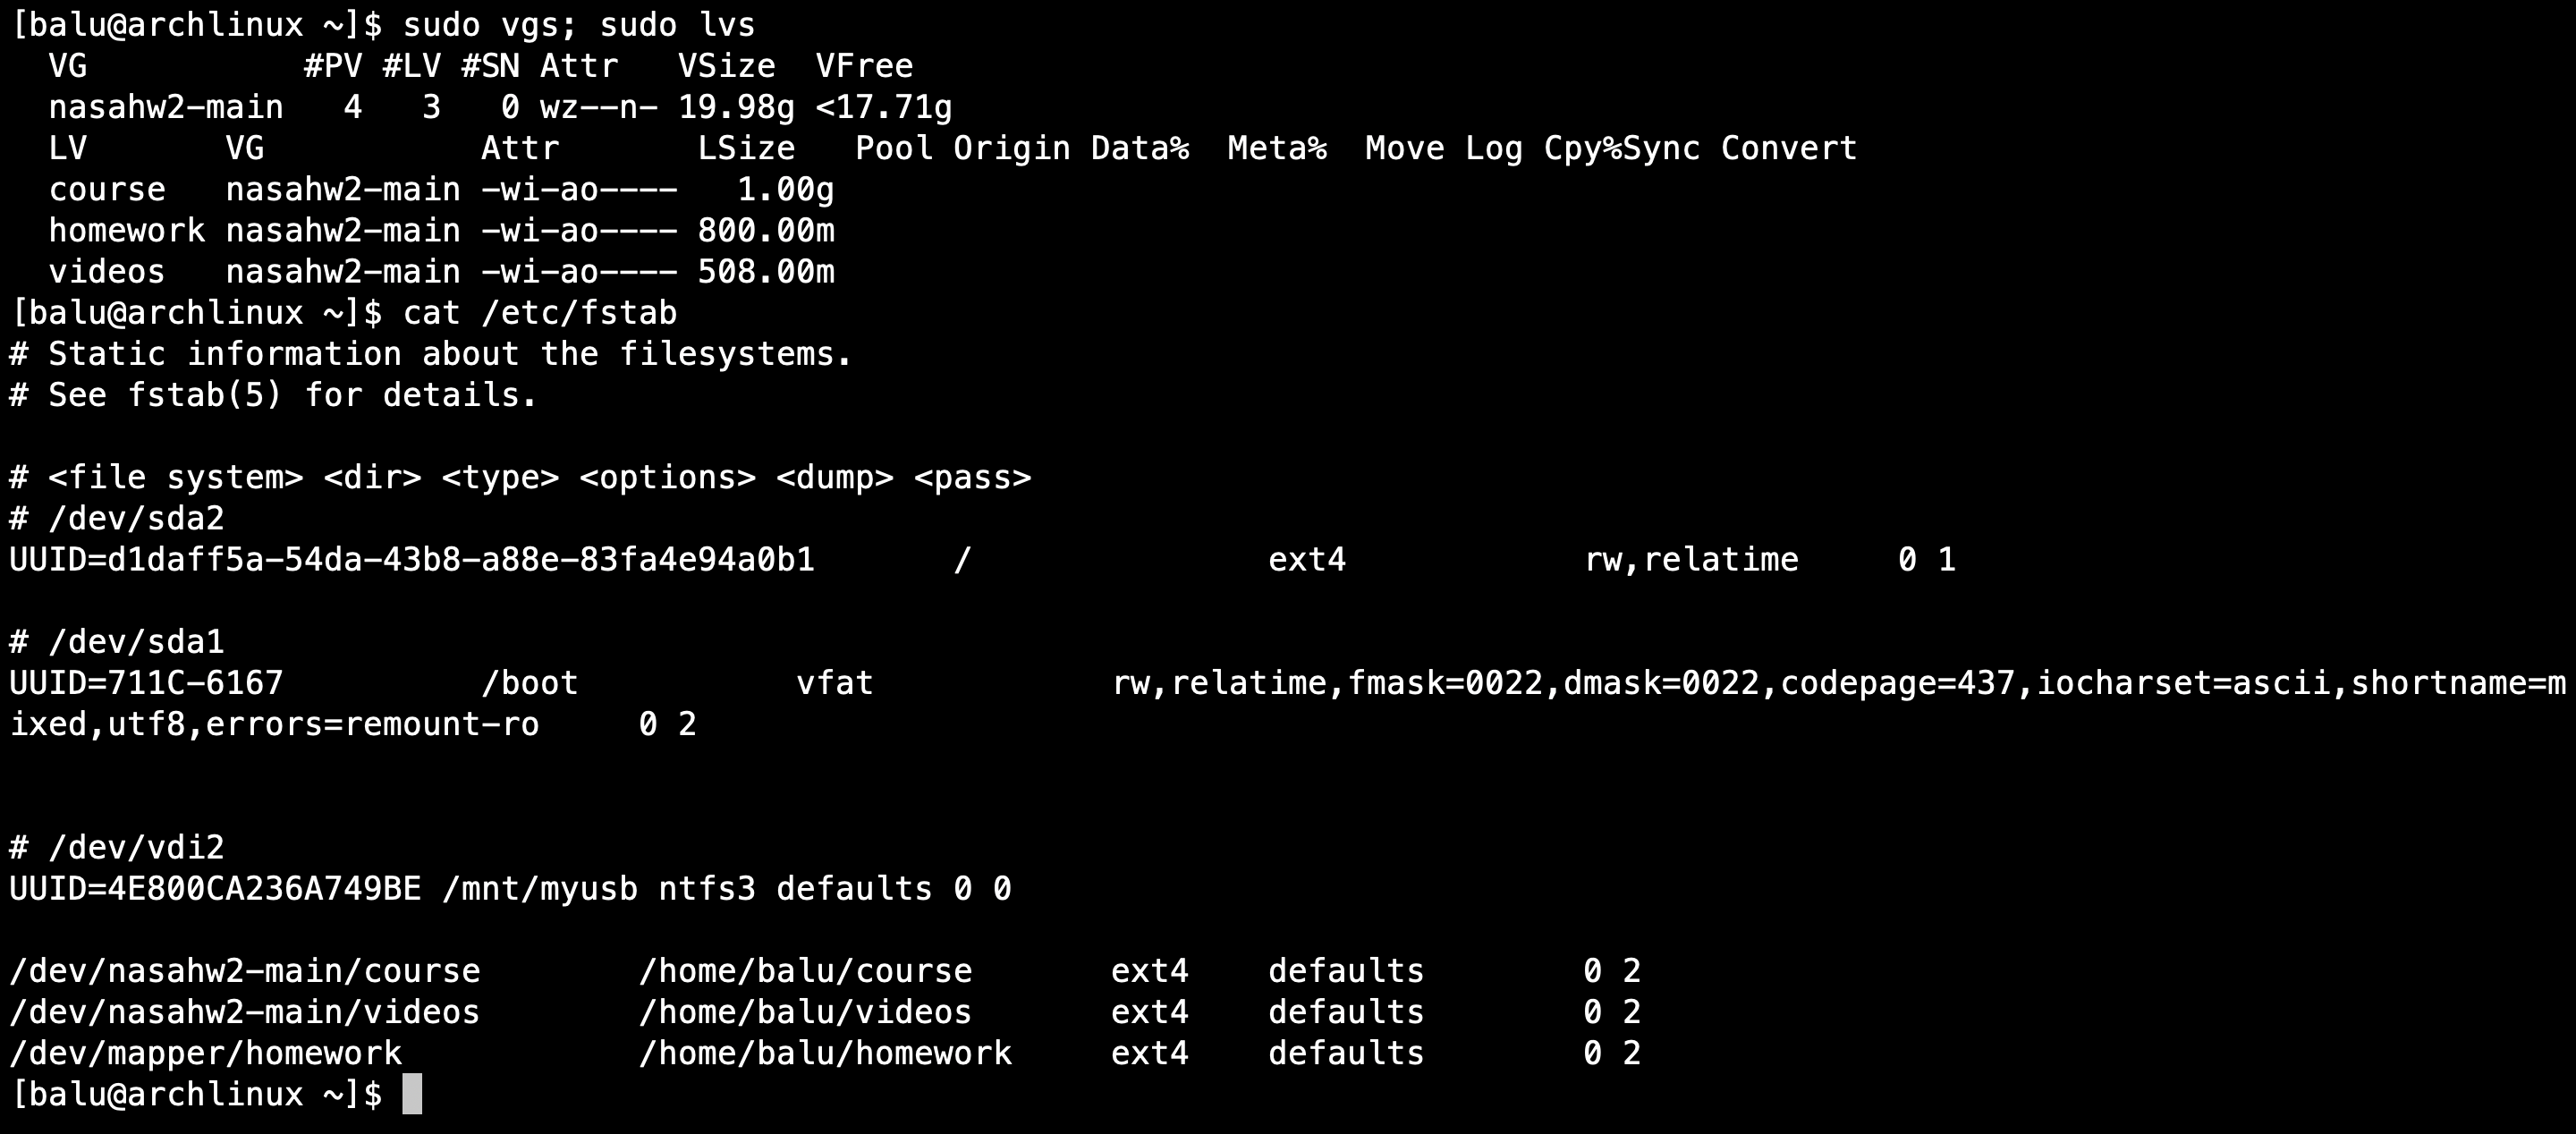
\includegraphics[width=0.99\textwidth]{images/7-3.png}
      \caption{Screenshot of \texttt{sudo vgs; sudo lvs} and \texttt{cat /ect/fstab}}
    \end{figure}
  \end{answer}
\end{mycolorbox}

% -----------------------------------------------------------
% Problem 8
\section{等一下，妳還沒回答我}
\begin{mycolorbox}[teal]
  \textbf{Reference:}
  \footnotesize
  \begin{enumerate}
    \item \href{https://www.ecscoupon.com/4536.html}{Btrfs 和 ZFS 區別是什麼，使用哪個比較好？}
    \item \href{https://blog.csdn.net/weixin_42792088/article/details/132862333}{初識 FUSE (CSDN)}
    \item \href{https://www.linwei.com.tw/forum-detail/76/}{磁碟分割MBR、GPT是什麼？}
    \item (a) \href{https://blog.darkthread.net/blog/1000-vs-1024-kb-kib/}{1000 還是 1024？KB、KiB、MB、MiB} \\
      (b) \href{https://superuser.com/questions/1741437/with-ls-sh-is-1k-a-kilobyte-a-kilobit-1000-bytes-1024-bytes-or-what}{With ls -sh, is 1K a kilobyte, a kilobit, 1000 bytes, 1024 bytes, or what?}
    \item \href{https://raidnas.tw/hsinchu-nas-raid-explain-rescue/}{5張圖輕鬆介紹RAID磁碟陣列}
  \end{enumerate}
\end{mycolorbox}

\begin{problem}{8.1}
  Btrfs 和 ZFS 都是支援 Copy On Write (CoW) 的檔案系統，但是 Btrfs 是 Linux 的內建檔案系統，而 ZFS 則是由 Sun Microsystems 開發的檔案系統。Btrfs 的特色是支援 RAID，而 ZFS 則是支援 RAID-Z。
\end{problem}

\begin{problem}{8.2}
  FUSE 是一種讓非 root 使用者不需要修改 kernel 當中的程式碼，即可以自己在使用者空間中實作檔案系統的技術。此技術的優點為方便開發與除錯檔案系統。缺點為效能較差。
\end{problem}

\begin{problem}{8.3}
  兩者皆為硬碟用於啟動系統的分割表格式。MBR 為 Master Boot Record 的縮寫，為舊的分割表格式，最多支援 2.1TB 的硬碟，且只支援最多 4 個主分割區，再多需要使用「擴展分區」。 GPT 為 GUID Partition Table 的縮寫，支援更大的硬碟，且可以切割成無限個分割區。(Windows 上只能 128 個)
\end{problem}

\begin{problem}{8.4} MB 採用 SI 制的定義，以 1000 進位。而 MiB 採用 IEC 的定義，以 1024 進位。
  \begin{itemize}
    \item 1 MB  = 1,000 KB  = 1,000,000 Bites ($1000 \times 1000$)
      \vspace{-0.3cm}
    \item 1 MiB = 1,024 KiB = 1,048,576 Bites ($1024 \times 1024$)
  \end{itemize}
  在工作站上，根據 GNU Coreutils ls manual page，使用 -h 時是以 1024 進位，顯示的為 MiB。若要以 1000 進位，則使用 \texttt{--si} 選項。
\end{problem}

\begin{problem}{8.5}

  RAID 全名為容錯式磁碟陣列，是將多顆硬碟透過虛擬化儲存技術，合併成一個或多個硬碟陣列組。
  \begin{itemize}
    \item RAID 0: 需要兩個以上的硬碟，將資料分割成多個區塊，並且分別寫入不同的硬碟，提高讀寫速度。然而，若其中一顆硬碟故障，則整個陣列的資料都會遺失，安全性較低。
    \item RAID 1: 需要兩個以上的硬碟，其中一個用來存放主資料，另一個作為鏡像備份，具有極高安全性，可以用來保存重要的關鍵資料。但成本、讀寫速度及硬碟空間利用率較低。
    \item RAID 5: 需要三個以上的硬碟，將資料分割成多個區塊，並且分別寫入不同的硬碟，並且在每個區塊中加入奇偶校驗碼，當其中一顆硬碟故障時，可以透過奇偶校驗碼重建資料。
    \item RAID 10: 需要四個以上的硬碟，將硬碟分成兩組。先將資料以 RAID 0 分別放在兩組，每組當中再以 RAID 1 做鏡像備份。缺點為成本較高，但具有高安全性和讀寫速度。
  \end{itemize}
\end{problem}

% -----------------------------------------------------------
%    You don't have to mess with anything below this line.
% -----------------------------------------------------------

\end{document}
